\chapter*{Chuyên đề 1. Lý thuyết Galois}
\addcontentsline{toc}{chapter}{Chuyên đề 1. Lý thuyết Galois}

Tài liệu tham khảo trong phần này lấy từ sách \cite{Judson2012} và trang youtube\footnote{\url{https://youtu.be/Buv4Y74_z7I?si=sQ0lOodnuLR0Yb00}}.

\section{Extension Fields}

\subsection*{Extension Fields}

\begin{definition}[Mở rộng trường (Extension Field)]
    Trường $E$ được gọi là \textbf{mở rộng trường} (hay \textbf{extension field}) của trường $F$ nếu $F$ là trường con của $E$. Khi đó $F$ được gọi là \textbf{trường cơ sở} (hay \textbf{base field}) và ký hiệu $F \subset E$.
\end{definition}

\begin{example}
    Trường nào nhỏ nhất chứa $\QQ$ và $\sqrt{2}$?

    Đáp án là trường $\QQ(\sqrt{2}) = \{ a + b \sqrt{2} : a, b \in \QQ \}$.

    Việc chứng minh $\QQ(\sqrt{2})$ là trường khá đơn giản, phần tử nghịch đảo đối với phép nhân của $a + b \sqrt{2}$ là
    \begin{equation*}
        \frac{a}{a^2 - 2 b^2} + \frac{-2b}{a^2 - 2 b^2} \sqrt{2}
    \end{equation*}
\end{example}

\begin{example}
    Trường nào nhỏ nhất chứa $\QQ$ và $i$ (ở đây $i$ là đơn vị ảo, $i^2 = -1$)?

    Đáp án là trường $\QQ(i) = \{ a + b i : a, b \in \QQ \}$. Tương tự, ở đây phần tử nghịch đảo đối với phép nhân của $a + b i$ là
    \begin{equation*}
        \frac{a}{a^2 + b^2} + \frac{-b}{a^2 + b^2} i
    \end{equation*}
\end{example}

Ở đây $\QQ(\sqrt{2})$ và $\QQ(i)$ đều là mở rộng của $\QQ$ và đều là tập con của $\CC$. Tuy nhiên hai trường này không phải tập con của nhau.

Như vậy, bằng việc mở rộng $\QQ$ với $\sqrt{2}$ ta có trường $\QQ(\sqrt{2})$.

Tương tự, bằng việc mở rộng $\QQ$ với $i$ ta có trường $\QQ(i)$.

Vậy trường nào chứa $\QQ$, $\sqrt{2}$ và $i$?

\begin{example}
    Trường chứa cả $\QQ$, $\sqrt{2}$ và $i$ là tập hợp
    \begin{equation*}
        \QQ(\sqrt{2}, i) = \{ a + b\sqrt{2} + c i + d \sqrt{2} i : a, b, c, d \in \QQ \}
    \end{equation*}
\end{example}

Trường trên có thể suy ra từ logic sau. Ta đã có $\QQ(i)$ chứa $\QQ$ và $i$. Ta muốn thêm $\sqrt{2}$ vào trường $\QQ(i)$ nên ta sẽ muốn mở rộng $\QQ(i)$ lên $\QQ(i)(\sqrt{2})$.

Khi đó $\QQ(i)(\sqrt{2})$ tương tự sẽ có dạng
\begin{equation*}
    \QQ(i)(\sqrt{2}) = \{ \alpha + \beta \sqrt{2} : \alpha, \beta \in \QQ(i) \}
\end{equation*}

Nói cách khác $\alpha = a + b i$ và $\beta = c + d i$, $a, b, c, d \in \QQ$, nên ta có
\begin{equation*}
    \alpha + \beta \sqrt{2} = a + b i + c \sqrt{2} + d \sqrt{2} i, \quad a, b, c, d \in \QQ
\end{equation*}

Khi đó ta viết
\begin{equation*}
    \QQ(i)(\sqrt{2}) = \QQ(\sqrt{2}, i) = \{ a + b\sqrt{2} + c i + d \sqrt{2} i : a, b, c, d \in \QQ \}
\end{equation*}

\begin{remark}
    \begin{enumerate}
        \item $\QQ(\sqrt{2})$ là trường con của $\RR$ nhưng $\QQ(i)$ không phải;
        \item $\QQ(i)$ nhỏ hơn $\CC$ rất nhiều (không chứa $\sqrt{2}$);
        \item $\QQ(\sqrt{2})$ chứa tất cả nghiệm của đa thức $f(x) = x^2 - 2$ trên $\QQ$. Do đó $\QQ(\sqrt{2})$ được gọi là \textbf{trường phân rã} của đa thức $f(x)$.
    \end{enumerate}
\end{remark}

\subsection*{Biểu diễn quan hệ giữa các trường qua lattice}

Ở phần trước, $\QQ(\sqrt{2})$ là mở rộng của $\QQ$ và với hai phần tử $a, b \in \QQ$ xác định một phần tử $a + b \sqrt{2} \in \QQ(\sqrt{2})$.

Do $a + b \sqrt{2} = a \cdot 1 + b \cdot \sqrt{2}$ nên $\{ 1, \sqrt{2} \}$ là \textbf{cơ sở} (hay \textbf{basis}) của $\QQ(\sqrt{2})$. Cơ sở chứa hai phần tử nên ta nói \textbf{bậc của mở rộng đơn} (hay \textbf{degree}) từ $\QQ$ lên $\QQ(\sqrt{2})$ là 2.

Tương tự, mở rộng từ $\QQ$ lên $\QQ(i)$ cũng có bậc là 2 với cơ sở là $(1, i)$.

Như vậy ta cũng các trường $\QQ(\sqrt{2})$, $\QQ(\sqrt{3})$ và $\QQ(\sqrt{6})$ là các mở rộng đơn bậc 2 của $\QQ$ (hình \ref{extension_field:1}).

\begin{figure}[htb]
    \centering
    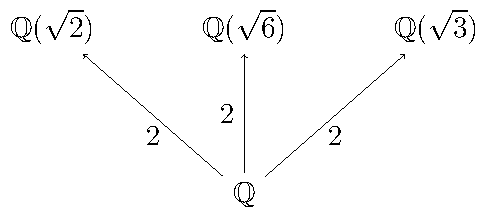
\includegraphics[page=1]{extension_field.pdf}
    \caption{Mở rộng trường $\QQ$ lên $\QQ(\sqrt{2})$, $\QQ(\sqrt{3})$ và $\QQ(\sqrt{6})$}
    \label{extension_field:1}
\end{figure}

Do $\sqrt{6} = \sqrt{2} \cdot \sqrt{3}$ dẫn ta tới câu hỏi, trường nào nhỏ nhất chứa cả $\sqrt{2}$ và $\sqrt{3}$?

Thực hiện tương tự với $\QQ(\sqrt{2}, i)$ ở trên ta có trường
\begin{equation*}
    \QQ(\sqrt{2}, \sqrt{3}) = \QQ(\sqrt{2})(\sqrt{3}) = \{ a + b \sqrt{2} + c \sqrt{3} + d \sqrt{6} : a, b, c, d \in \QQ \}
\end{equation*}
là trường nhỏ nhất chứa cả $\sqrt{2}$ và $\sqrt{3}$.

Ở đây, $\QQ(\sqrt{2}, \sqrt{3})$ là mở rộng bậc 4 của $\QQ$ với cơ sở là $\{ 1, \sqrt{2}, \sqrt{3}, \sqrt{6} \}$.

Bằng việc mở rộng từ $\QQ(\sqrt{2})$ lên $\QQ(\sqrt{2}, \sqrt{3}) = \QQ(\sqrt{2})(\sqrt{3})$ ta cũng có đây là mở rộng bậc 2 (tương tự chứng minh phía trên cho $\QQ(\sqrt{2}, i)$). Như vậy mở rộng từ $\QQ(\sqrt{3})$ lên $\QQ(\sqrt{2}, \sqrt{3})$ cũng là mở rộng bậc 2.

Vậy mở rộng từ $\QQ(\sqrt{6})$ lên $\QQ(\sqrt{2}, \sqrt{3})$ là bậc mấy? Để xác định ta cần chứng minh nhận xét sau

\begin{remark}
    $\QQ(\sqrt{2}, \sqrt{3}) \equiv \QQ(\sqrt{2} + \sqrt{3})$, trong đó $\QQ(\sqrt{2} + \sqrt{3})$ là trường nhỏ nhất chứa $\QQ$ và $\sqrt{2} + \sqrt{3}$.
\end{remark}

\begin{proof}
    Ta chứng minh $\QQ(\sqrt{2}, \sqrt{3}) \subset \QQ(\sqrt{2} + \sqrt{3})$.

    Do $\sqrt{2} + \sqrt{3}$ nên nghịch đảo $\dfrac{1}{\sqrt{2} + \sqrt{3}} = \sqrt{3} - \sqrt{2} \in \QQ(\sqrt{2} + \sqrt{3})$.

    Khi đó, $\dfrac{1}{2} \cdot (\sqrt{2} + \sqrt{3}) \pm \dfrac{1}{2} \cdot (\sqrt{3} - \sqrt{2}) \in \QQ(\sqrt{2} + \sqrt{3})$.

    Vế trái sẽ bằng $\sqrt{2}$ hoặc $\sqrt{3}$. Như vậy $\sqrt{2}, \sqrt{3} \in \QQ(\sqrt{2} + \sqrt{3})$.

    Phép nhân trên trường cho ta $\sqrt{2} \cdot \sqrt{3} = \sqrt{6} \in \QQ(\sqrt{2} + \sqrt{3})$.

    Như vậy với mọi $a, b, c, d \in \QQ$ ta có $a + b \sqrt{2} + c \sqrt{3} + d \sqrt{6} \in \QQ(\sqrt{2} + \sqrt{3})$. Điều này tương đương với $\QQ(\sqrt{2}, \sqrt{3}) \subset \QQ(\sqrt{2} + \sqrt{3})$.

    Nhưng mà $\QQ(\sqrt{2} + \sqrt{3})$ là trường nhỏ nhất chứa $\QQ$ và $\sqrt{2} + \sqrt{3}$, và $\QQ(\sqrt{2}, \sqrt{3})$ là trường nhỏ nhất chứa $\sqrt{2}$ và $\sqrt{3}$, kéo theo chứa cả $\sqrt{2} + \sqrt{3}$ nên $\QQ(\sqrt{2} + \sqrt{3}) \equiv \QQ(\sqrt{2}, \sqrt{3})$.
\end{proof}

Ta có $\QQ(\sqrt{6}) = \{ a + b \sqrt{6} : a, b \in \QQ \}$. Khi đó
\begin{equation}
    \label{QQ6_to_QQ2+3}
    \QQ(\sqrt{6})(\sqrt{2} + \sqrt{3}) = \{ \alpha + \beta (\sqrt{2} + \sqrt{3}) : \alpha, \beta \in \QQ(\sqrt{6}) \}
\end{equation}

Đặt $\alpha = a + b \sqrt{6}$ và $\beta = c + d \sqrt{6}$, như vậy mỗi phần tử trong $\QQ(\sqrt{6})(\sqrt{2} + \sqrt{3})$ có dạng
\begin{align*}
    a + b \sqrt{6} + (c + \sqrt{6})(\sqrt{2} + \sqrt{3}) = & a + (c + 3d) \sqrt{2} + (c + 2d) \sqrt{3} + b \sqrt{6} \\
        = & a' + b' \sqrt{2} + c' \sqrt{3} + d' \sqrt{6}
\end{align*}
với $a \to a'$, $c+3d \to b'$, $c + 2d \to c'$ và $b \to d'$.

Biến đổi này tương đương với hệ phương trình tuyến tính
\begin{equation*}
    \begin{pmatrix}
        1 & 0 & 0 & 0 \\
        0 & 0 & 1 & 3 \\
        0 & 0 & 1 & 2 \\
        0 & 1 & 0 & 0
    \end{pmatrix} \begin{pmatrix}
        a \\ b \\ c \\ d
    \end{pmatrix} = \begin{pmatrix}
        a' \\ b' \\ c' \\ d'
    \end{pmatrix}
\end{equation*}

Ma trận trên khả nghịch trên $\QQ$, do đó $\QQ(\sqrt{6})(\sqrt{2} + \sqrt{3}) \equiv \QQ(\sqrt{2}, \sqrt{3})$. Ở dạng biểu diễn \ref{QQ6_to_QQ2+3} ta suy ra mở rộng từ $\QQ(\sqrt{6})$ lên $\QQ(\sqrt{2}, \sqrt{3})$ là mở rộng bậc 2.

Sơ đồ mở rộng trường bây giờ như sau

\begin{figure}[htb]
    \centering
    \includegraphics[page=2]{extension_field.pdf}
\end{figure}

\subsection*{Splitting Field}

\begin{definition}[Trường phân rã (Splitting Field)]
    Xét trường $F$ và đa thức khác hằng $p(x) = a_n x^n + a_{n-1} x^{n-1} + \ldots + a_1 x + a_0$ trên $F[x]$ ($a_i \in F$ với mọi $i = 1, 2, \ldots$).

    Trường mở rộng $E$ của trường $F$ được gọi là \textbf{trường phân rã} (hay \textbf{splitting field}) của $p(x)$ nếu tồn tại các phần tử $\alpha_1, \alpha_2, \ldots, \alpha_n$ thuộc $E$ sao cho $E = F(\alpha_1, \alpha_2, \ldots, \alpha_n)$ và
    \begin{equation*}
        p(x) = (x - \alpha_1) (x - \alpha_2) \cdots (x - \alpha_n)
    \end{equation*}
\end{definition}

Khi đó ta nói đa thức $p(x) \in F[x]$ phân rã (split) trong $E$ nếu nó phân tích thành các nhân tử bậc nhất (tuyến tính) trong $E[x]$.

Nói nôm na, nếu đa thức có hệ số trong một trường $F$ nào đó (tức thuộc $F[x]$) thì các nghiệm của nó nằm trong một trường lớn hơn chứa $F$.

\begin{example}
    Đa thức $f(x) = x^2 - 2$ trên $\QQ[x]$ không có nghiệm trên $\QQ$. Tuy nhiên $\QQ(\sqrt{2})$ là trường chứa $\QQ$ và các nghiệm của $f(x)$ là $\pm \sqrt{2}$. Vì vậy $\QQ(\sqrt{2})$ là trường phân rã của $f(x)$.
\end{example}

\begin{example}
    Đa thức $g(x) = x^2 + i$ trên $\QQ[x]$ không có nghiệm trên $\QQ$. Tuy nhiên $g(x)$ có hai nghiệm là $\pm i$ và $\QQ(i)$ chứa cả $\QQ$ và $\pm i$ nên $\QQ(i)$ là một trường phân rã của $g(x)$.
\end{example}

Ở đây, bậc của đa thức $f(x) = x^2 - 2$ bằng với bậc của mở rộng trường từ $\QQ$ lên $\QQ(\sqrt{2})$.

Tương tự, bậc của mở rộng trường từ $\QQ$ lên $\QQ(\sqrt{3})$ bằng bậc đa thức $g(x) = x^2 - 3$, và bậc của mở rộng trường từ $\QQ$ lên $\QQ(\sqrt{6})$ bằng với bậc đa thức $h(x) = x^2 - 6$.

Ở trên ta đã chứng minh bậc của mở rộng trường từ $\QQ(\sqrt{2})$ lên $\QQ(\sqrt{2}, \sqrt{3})$ là 2, điều này tương ứng với bậc của đa thức $k(x) = (x^2 - 2)(x^2 - 3) = x^4 - 5 x + 6$.

Tổng kết lại, nếu $E$ là trường phân rã của $F$ trên đa thức $f(x) \in F[x]$ thì bậc của mở rộng trường từ $F$ lên $E$ bằng với bậc của $f(x)$.

Từ sơ đồ mở rộng trường bên trên ta có sơ đồ với đa thức tương ứng.

\begin{figure}[htb]
    \centering
    \includegraphics[page=3]{extension_field.pdf}
\end{figure}

Vậy còn mở rộng từ $\QQ(\sqrt{6})$ thành $\QQ(\sqrt{2}, \sqrt{3})$? Ở trên ta đã chứng minh rằng đây là mở rộng bậc 2. Vậy chúng ta cần tìm một đa thức bậc 2 có hệ số trong $\QQ(\sqrt{6})$ mà không có nghiệm trong $\QQ(\sqrt{6})$.

Quay lại một chút, ta đã mở rộng $\QQ(\sqrt{6})$ lên $\QQ(\sqrt{2}, \sqrt{3})$ với sự trợ giúp của phần tử $\sqrt{2} + \sqrt{3}$. Từ đây ta có thể xây dựng đa thức
\begin{equation*}
    m(x) = x^2 - (\sqrt{2} + \sqrt{3})^2 = x^2 - 5 - 2 \sqrt{6}
\end{equation*}

Đa thức $m(x)$ có hệ số trong $\QQ(\sqrt{6})$ nhưng không có nghiệm trong $\QQ(\sqrt{6})$ mà trong $\QQ(\sqrt{2}, \sqrt{3})$. Ta có điều phải chứng minh.
